\documentclass{article}

\usepackage[utf8]{inputenc}

\usepackage{nicefrac}
\usepackage{amssymb, amsmath, amsfonts}
\usepackage{amsthm}
\usepackage{tikz}
\usetikzlibrary{matrix,shapes,arrows, calc, intersections}
\usepackage{pgfplots}
\usepgfplotslibrary{groupplots}
\usepackage[a4paper, margin=1in]{geometry}

\newtheorem{proposition}{Proposition}
\newtheorem{theorem}{Theorem}
\newtheorem{definition}{Definition}
\newtheorem{lemma}{Lemma}
\newtheorem{conjecture}{Conjecture}
\newtheorem{corollary}{Corollary}
\newtheorem{remark}{Remark}
\newtheorem{assumption}{Assumption}

\newlength\figureheight
\newlength\figurewidth
\setlength\figureheight{12cm}
\setlength\figurewidth{14cm}

\newcommand{\tikzdir}[1]{tikz/#1.tikz}
\newcommand{\inputtikz}[1]{\input{\tikzdir{#1}}}

\DeclareMathOperator*{\argmin}{arg\; min}     % argmin
\DeclareMathOperator*{\argmax}{arg\; max}     % argmax
\DeclareMathOperator*{\tr}{tr}     % trace
\DeclareMathOperator{\Cov}{Cov}
\DeclareMathOperator{\logdet}{log\;det}

\title{EE8087 Living with Mathematics\\Tutorial 1: Trigonometry}
\date{}
\begin{document} \maketitle
\begin{enumerate}
\item In a circle of radius 6 cm, a triangle PQR is drawn having QR=$8$ and PQ=$10$. What is the length of PR?

  \begin{figure}[ht]
    \centering
    \begin{tikzpicture}[scale=0.5]
      \tikzset{mark coordinate/.style={inner sep=0pt,
          outer sep=0pt,
          minimum size=3pt,
          fill=#1,
          circle}
      }
      \node [mark coordinate=black,label=$O$] (O) at (0,0) {}; 
      \node [mark coordinate=black,label=50:$Q$] (Q) at (6,0) {}; 
      \draw [name path=Circle, thick] (O) circle (6cm);
      \path [name path=Circle1] (Q) circle (8cm);
      \path [name path=Circle2] (Q) circle (10cm);

      \path [name intersections={of=Circle and Circle1, name=i}] (i-1) coordinate [mark coordinate=black, label=$R$];
      \path [name intersections={of=Circle and Circle2, name=j}] (j-2) coordinate [mark coordinate=black, label=270:$P$];
      \draw [thick] (i-1) -- (j-2) -- (Q) -- (i-1) ;
    \end{tikzpicture}
    \caption{Question 1}
  \end{figure}

\item  An engineer determines that the angle of elevation from her position to the top of a tower is $52^o$ . She measures the angle of elevation again from a point $47$ m further away from position and finds it to be $31^o$ . Both positions are due east of the tower. Find the height of the tower.

   \begin{figure}[ht]
    \centering
    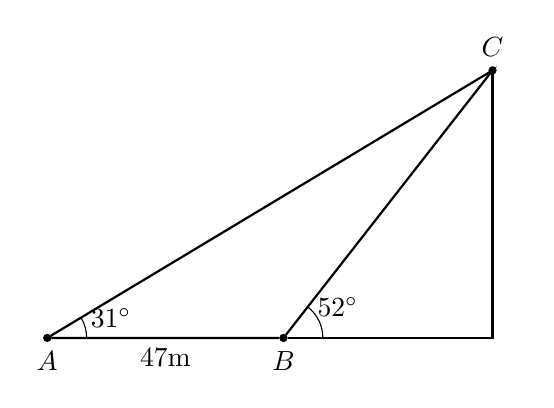
\begin{tikzpicture}[scale=0.5]
      \tikzset{mark coordinate/.style={inner sep=0pt,
          outer sep=0pt,
          minimum size=3pt,
          fill=#1,
          circle}
      }
      \node [mark coordinate=black,label=270:$A$] (A) at (0,0) {}; 
      \node [mark coordinate=black,label=270:$B$] (B) at (6,0) {}; 
      \coordinate (A1) at ($(A)+(31:14)$);
      \coordinate (B1) at ($(B)+(52:10)$);
      \path [name path=AC] (A)--(A1);
      \path [name path=BC] (B)--(B1);
      \path [name intersections={of=AC and BC, by=C}];
      \node [mark coordinate=black, label=90:$C$] at (C) {};
      \draw [thick] (A)--(C)--(B)--node [below]{$47$m} (A);
      \draw [thick] (C)--(C)|-(B)--(B);

      \draw (1,0) arc (0:31:1) node [right] {$31^\circ$};
      \draw (7,0) arc (0:52:1) node [right] {$52^\circ$};

    \end{tikzpicture}
    \caption{Question 2}
  \end{figure}
 
  
\newpage

  
\item Two towers, whose tops are labeled as P and Q, are of the same height. They are $4.1$ km apart on level ground. A pilot measures the angle of depressions to P and Q to be $36.5^o$ and $25^o$ , respectively. Find the height of the airplane from the top of the towers.

   \begin{figure}[ht]
    \centering
    \begin{tikzpicture}[scale=0.5]
      \tikzset{mark coordinate/.style={inner sep=0pt,
          outer sep=0pt,
          minimum size=3pt,
          fill=#1,
          circle}
      }
      \node [mark coordinate=black,label=270:$Q$] (A) at (0,0) {}; 
      \node [mark coordinate=black,label=270:$P$] (B) at (6,0) {}; 
      \coordinate (A1) at ($(A)+(25:14)$);
      \coordinate (B1) at ($(B)+(36.5:10)$);
      \path [name path=AC] (A)--(A1);
      \path [name path=BC] (B)--(B1);
      \path [name intersections={of=AC and BC, by=C}];
      \node [mark coordinate=black, label=90:$C$] at (C) {};
      \draw [thick] (A)--(C)--(B)--node [below]{$4.1$km} (A);
      \draw [dashed] (C)|-(B)--(B);

      \draw (1,0) arc (0:31:1) node [right] {$25^\circ$};
      \draw (7,0) arc (0:52:1) node [right] {$36.5^\circ$};

    \end{tikzpicture}
    \caption{Question 4}
  \end{figure}
 
\item  In a triangle ABC, angle A is trisected by segments AE and AD where points E and D lie on BC. Let BD = $2$cm, DE = $3$cm and EC = $6$cm. Find the length of the shortest side of the triangle ABC.
    \begin{figure}[ht]
    \centering
    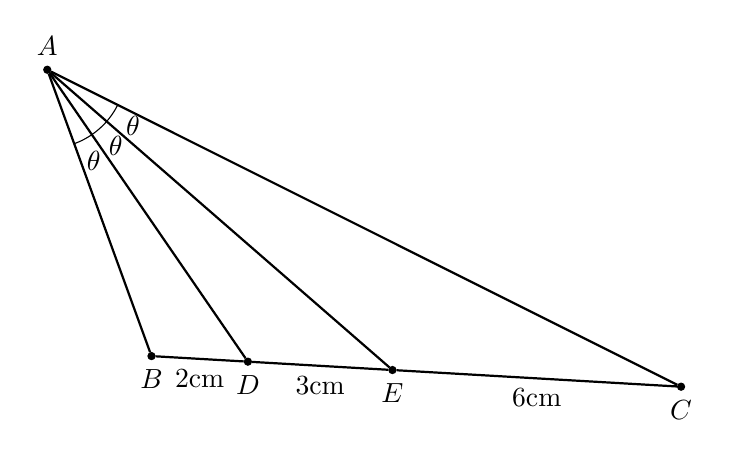
\begin{tikzpicture}[scale=1]
      \tikzset{mark coordinate/.style={inner sep=0pt,
          outer sep=0pt,
          minimum size=3pt,
          fill=#1,
          circle}
      }
      \node [mark coordinate=black,label=90:$A$] (A) at (0,0) {}; 
      \node [mark coordinate=black,label=270:$B$] (B) at (-70:3.87) {};
      \node [mark coordinate=black,label=270:$C$] (C) at (-26.57:9) {};

      \node [mark coordinate=black,label=270:$D$] (D) at ($(B)!.182!(C)$) {};
      \node [mark coordinate=black,label=270:$E$] (E) at ($(B)!.455!(C)$) {};

      \draw [thick] (A)--(B)-- node [below] {$2$cm} (D)
      -- node [below] {$3$cm} (E)
      -- node [below] {$6$cm} (C)--(A);
      \draw [thick] (A)--(D);
      \draw [thick] (A)--(E);
      \draw (-70:1) arc (-70:-26.57:1);
      \node at (-63:1.3) {$\theta$};
      \node at (-48:1.3) {$\theta$};
      \node at (-33:1.3) {$\theta$};
    \end{tikzpicture}
    \caption{Question 4}
  \end{figure}
  
\item You have a pizza of radius $25$ cm.The pizza was cut into $16$ equal slices. When only one slice was left, your brother and you both wanted it. So, both of you agreed to cut it into two halves but you like the crust more than your brother does. So, you decided to cut it in a way shown in Fig~\ref{fig:5}. How far up the radius from the center of the circle will you need to cut so that both will have an equal area of the pizza.
   \begin{figure}[ht]
    \centering
    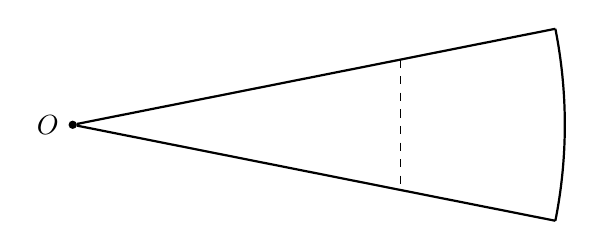
\begin{tikzpicture}[scale=0.25]
      \tikzset{mark coordinate/.style={inner sep=0pt,
          outer sep=0pt,
          minimum size=3pt,
          fill=#1,
          circle}
      }
      \node [mark coordinate=black,label=180:$O$] (O) at (0,0) {}; 
      \draw [thick] (11.25:25)--(O)--(-11.25:25);
      \draw [thick] (11.25:25) arc (11.25:-11.25:25);

      \draw [dashed] (11.25:17)-- (-11.25:17);

    \end{tikzpicture}
    \caption{Question 5\label{fig:5}}
  \end{figure}
 
\end{enumerate}

\end{document}
%%% Local Variables:
%%% TeX-command-default: "Latexmk"
%%% End:
